\subsubsection*{T1.4 System dynamics estimation software. Extension to
environmental compliance estimation (..., TUD 2PM, ...)}

During year two, TUD worked with the WBI toolbox in Matlab to study whole-body controllers capable of integrating learned inverse dynamics models. The idea, more specifically, is to combine the low-level torque control at joint level with the learned dynamics models of WP4 (T4.2), which can thus provide the correct torques for rigid and compliant contacts. TUD implemented a whole-body impedance controller and two balance controllers with the WBI toolbox in Matlab (see Figure~\ref{fig:wbitud}). The controllers were tested on Gazebo and on the iCub mex model simulated in Matlab. The integration with the outcome of WP4 is ongoing.

 \begin{figure}
 \centering
 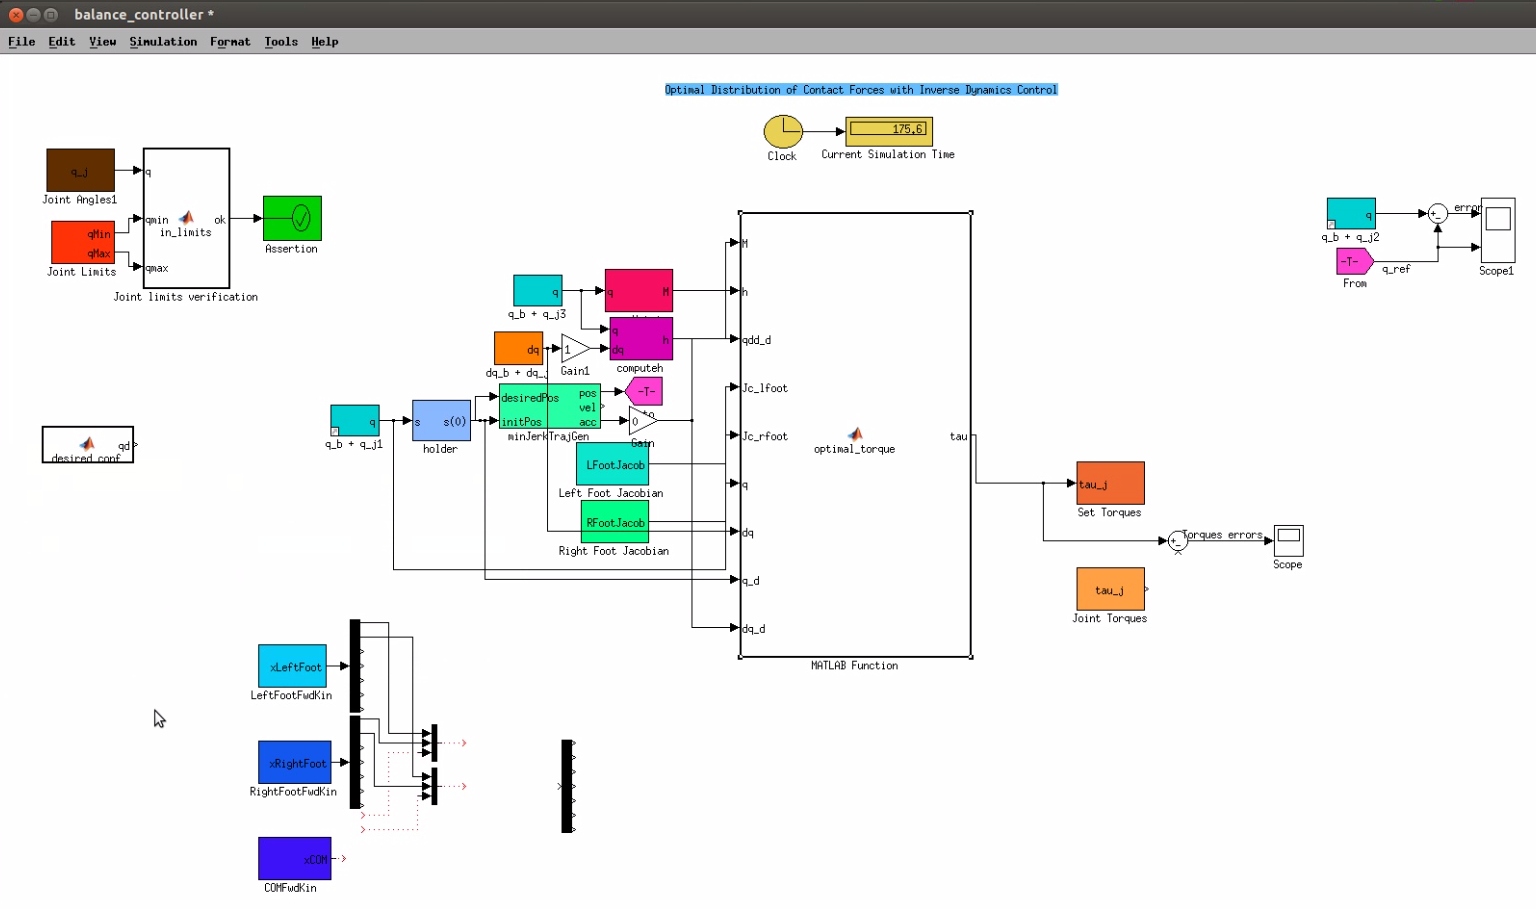
\includegraphics[width=0.7\textwidth]{wbi_torque_controller.png}
  \caption{One of the balance controllers implemented by TUD with the WBI toolbox in Matlab. 
 }
 \label{fig:wbitud}
 \end{figure}


%cite your papers \cite{ivaldi2014simulators}

% started to investigate the learning of dynamic models with
% discontinuities. A new Gaussian process (GP) model was developed
% that is explicitly designed to deal with non-linearities
% induced through contacts with the environment. An example of such non-linearities 
% and the approximated model reconstruction is shown in Figure \ref{fig:example_discontinuities}.
% We called the developed supervised learning method manifold GP (mGP), as it 
% jointly learns a transformation of the data into a feature space, and a GP regression 
%  from the feature space to observed space. In future work, this promising approach 
%  will be applied to motor skill learning task on the iCub with multiple contacts. 
%  A preprint of this work 
%  was published this year [Calandra, R. and Peters, J. and Rasmussen, C. and Deisenroth,
% M., 2014].
% 
% \begin{figure}
% \centering
% 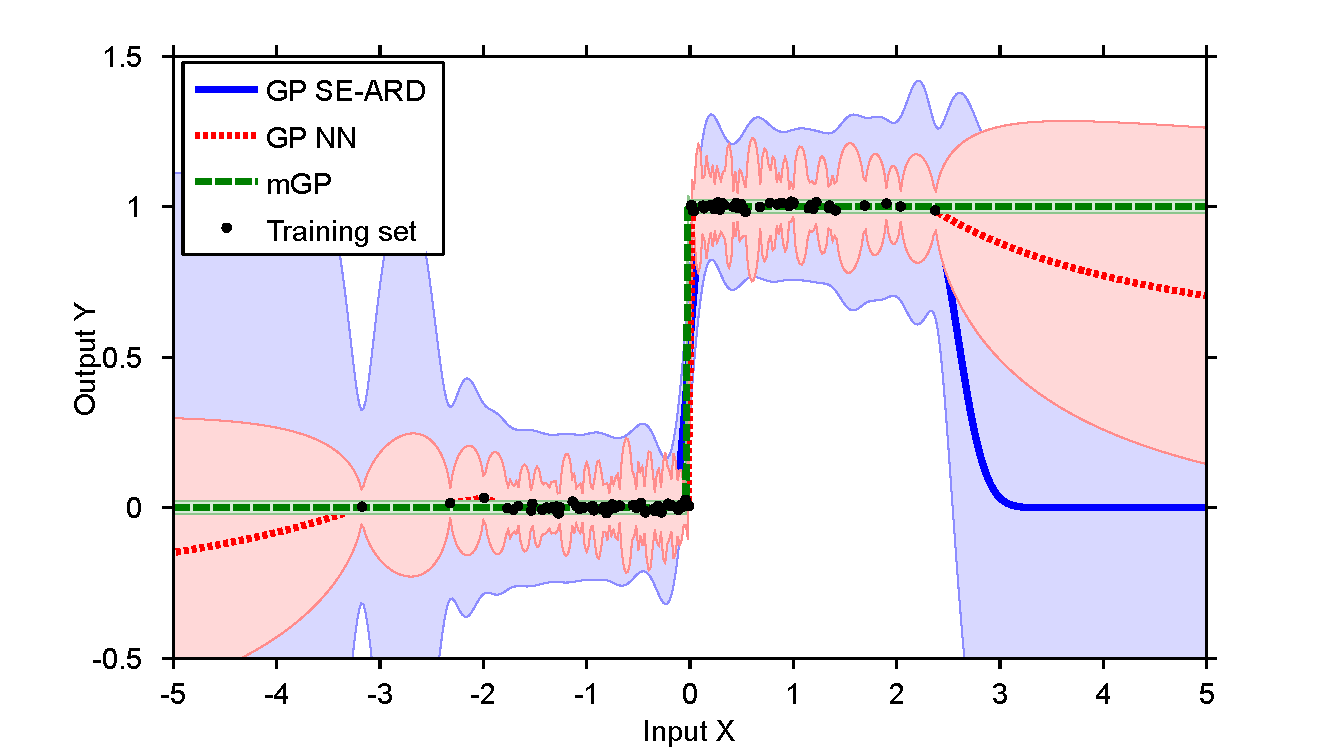
\includegraphics[width=0.7\textwidth]{./pics_tud/AAAI2014_0.pdf}
% %\label{fig:subfig2}
%  \caption{Illustration of a discontinuous function (black dots) that is approximated by three 
%  model learning approaches. Classical Gaussian process regression methods (GP SE-ARD, and GP NN) 
%  poorly reconstruct this function as they average over the ``jump'', which results in a high model variance. 
%  TUD, however, demonstrated that by jointly learning a transformation of the data into a feature space, 
%  and a GP regression model from the feature space to observed space, the non-linear function 
%  can be reconstructed without large reconstruction errors. 
% }
% \label{fig:example_discontinuities}
% \end{figure}